\documentclass[10pt]{article}
\usepackage{caption}
\usepackage{tabularx}
\usepackage{amsmath, amsfonts, amsthm, amssymb, mathrsfs}  % Some math symbols
\usepackage{bbold}
\usepackage{dsfont}
\usepackage{bm}
\usepackage{enumerate}
\usepackage{enumitem}
\usepackage{fullpage}
\usepackage{hyperref}
\usepackage{mathtools}
\usepackage{listings}
\usepackage{tikz}
\usepackage{tkz-euclide}
\usepackage{xcolor}
\usepackage{multicol}
\usepackage[margin=0.8in]{geometry}
\usepackage{lastpage}
\usepackage{fixltx2e}
\usepackage{pgfplots}
\usepackage{xcolor}
\usepackage{colortbl}
\usepackage{tcolorbox}
\usetikzlibrary{intersections}
\usetikzlibrary{positioning}
\usetikzlibrary{shapes}
\usepgfplotslibrary{fillbetween}
\tikzset{>=latex}

%%%%%%%%%%%%%%%%%%%%%SETTING%%%%%%%%%%%%%%%%%%%%%%
%Nope sick of it now
%\renewcommand*\familydefault{\sfdefault} %% Only if the base font of the document is to be sans serif
%Listing
\lstset{
    language=SQL,
	numbers=left,
	basicstyle=\ttfamily\footnotesize,
	breaklines=true
}
%Indent
\def\indented#1{\list{}{}\item[]}
\let\indented=\endlist
%%%%%%%%%para indent/skip%%%%%%%%%%%
\setlength{\parindent}{0pt}
\setlength{\parskip}{8pt plus 1pt}
\setlength{\multicolsep}{6.0pt plus 2.0pt minus 1.5pt}% 50% of original values
%%%%%%%%%Bracket%%%%%%%%%%%%%%%
\newcommand{\bracket}[1]{\left[#1\right]}
\newcommand{\parenth}[1]{\left(#1\right)}
\newcommand{\matrices}[1]{\begin{bmatrix}#1\end{bmatrix}}
\newcommand{\indicator}[1]{\mathbb{1}\left\{#1\right\}}
%%%%%%%%%highlight%%%%%%%%%%%%%%%%
\newcommand{\highlight}[1]{\colorbox{yellow}{$\displaystyle #1$}}
\DeclareMathOperator*{\argmin}{arg\,min}
\DeclareMathOperator*{\argmax}{arg\,max}
%%%%%%%%%table%%%%%%%%%%%%%%%%
\newcolumntype{Y}{>{\centering\arraybackslash}X}
\def\tabularxcolumn#1{m{#1}}
%%%%%%%%%%%title%%%%%%%%%%%%%%%%%%%%%%%
\newcommand{\myname}{Linxing Preston Jiang}
\newcommand{\quarter}{Autumn 2017}
\newcommand{\myhwname}{\textbf{CSE 344: Homework 7}}
%%%%%%%%%%%my color box%%%%%%%%%%
\newtcolorbox{mybox}{colback=purple!20,colframe=purple!20}
%%%%%%%%%%%%%%%%%%%%%%%%%%%%FILE%%%%%%%%%%%%%%%%%%%%%%%%%%%%%%%%%%%%
\begin{document}
\begin{center}
	{\Large \myhwname} \\
	\vspace{.05in} 
    \myname\quad\quarter \\
	\vspace{.05in} 
    \today \\
\end{center}
\vspace{.15in} \hrule \vspace{0.5em}%

\begin{enumerate}[label=\textbf{\arabic*.}, listparindent=0.0em, itemsep=1em]
    % #1 
    \item E/R Graph: \\
    \begin{center}
        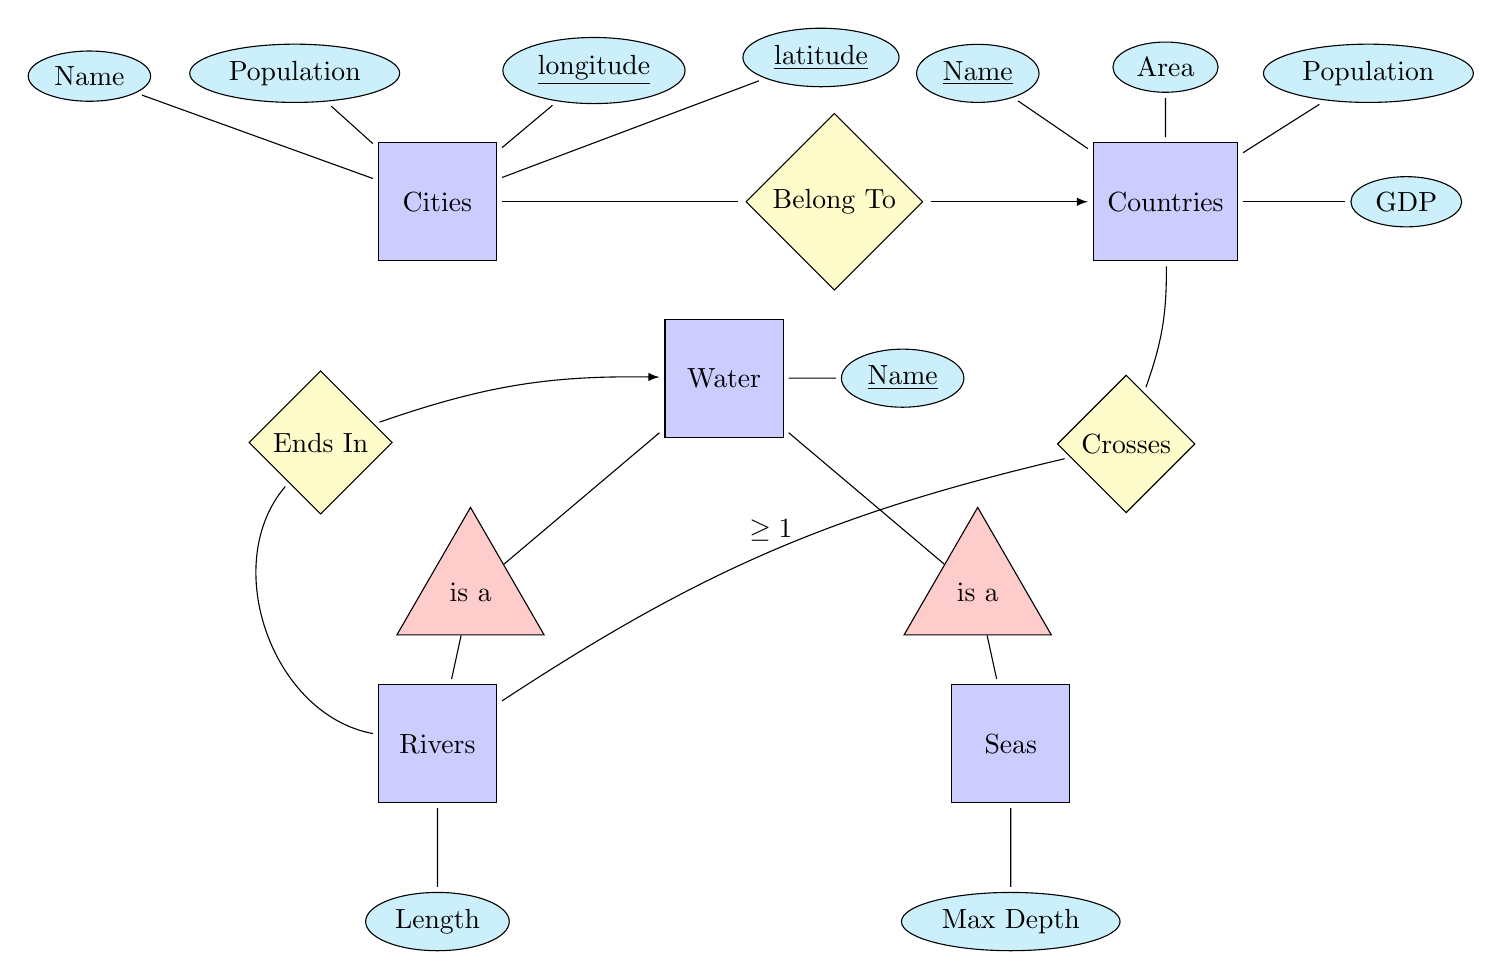
\begin{tikzpicture}[
            table/.style={rectangle, draw, fill=blue!20, minimum size=15mm, inner sep=5pt, outer sep=2pt},
            relation/.style={diamond, draw, fill=yellow!20, minimum size=3mm, inner sep=3pt, outer sep=2pt},
            attr/.style={ellipse, draw, fill=cyan!20, minimum size=5mm, inner sep=3pt, outer sep=2pt}, 
            subclass/.style={regular polygon, regular polygon sides=3, draw, fill=red!20},
            scale=0.6
        ]
        \node[table] (cities) at (-15, 0) {Cities};
        \node[attr, above left = 0.5cm and 3cm of cities] (cityname) {Name};
        \node[attr, above left = 0.5cm and 0cm of cities] (citypopulation) {Population};
        \node[attr, above right = 0.5cm and 0.3cm of cities] (longitude) {\underline{longitude}};
        \node[attr, above right = 0.7cm and 3.3cm of cities] (latitude) {\underline{latitude}};
        \path (cities) edge (cityname);
        \path (cities) edge (citypopulation);
        \path (cities) edge (longitude);
        \path (cities) edge (latitude);
        \node[relation, right = 3cm of cities] (belong) {Belong To};
        \path (cities) edge (belong);
        \node[table, right = 2cm of belong] (countries) {Countries};
        \path[->] (belong) edge (countries);
        \node[attr, above left = 0.5cm and 0.8cm of countries] (countryname) {\underline{Name}};
        \node[attr, above = 0.5cm of countries] (countryarea) {Area};
        \node[attr, above right = 0.5cm and 0.6cm of countries] (countrypopulation) {Population};
        \node[attr, right = 1.3cm of countries] (countrygdp) {GDP};
        \path (countries) edge (countryname);
        \path (countries) edge (countryarea);
        \path (countries) edge (countrypopulation);
        \path (countries) edge (countrygdp);
        \node[table, below right = 0.6cm and 2cm of cities] (water) {Water};
        \node[attr, right = 0.6cm of water] (watername) {\underline{Name}};
        \path (water) edge (watername);
        \node[subclass, below left = 1.5cm and 2cm of water] (isariver) {is a};
        \node[subclass, below right = 1.5cm and 2cm of water] (isasea) {is a};
        \path (water) edge (isariver);
        \path (water) edge (isasea);
        \node[table, below left = 3cm and 2cm of water] (river) {Rivers};
        \node[table, below right = 3cm and 2cm of water] (sea) {Seas};
        \path (isariver) edge (river);
        \path (isasea) edge (sea);
        \node[attr, below = 1cm of river] (riverlength) {Length};
        \node[attr, below = 1cm of sea] (seadepth) {Max Depth};
        \path (river) edge (riverlength);
        \path (sea) edge (seadepth);
        \node[relation, above left = 1cm and 1cm of isariver] (endsin) {Ends In};
        \path (river) edge[bend left=60] (endsin);
        \path[->] (endsin) edge[bend left=10] (water);
        \node[relation, above right= 1cm and 1cm of isasea] (cross) {Crosses};
        \path (river) edge[bend left=10] node[above, midway] {$\geq 1$} (cross);
        \path (cross) edge[bend right=10] (countries);
        \end{tikzpicture}
    \end{center}
    % #2
    \item 
        \begin{itemize}
            \item See the queries below.
            \begin{lstlisting}
CREATE TABLE InsuranceCo (name varchar(20) PRIMARY KEY, phone integer);
CREATE TABLE Person (ssn integer PRIMARY KEY, name varchar(20));
CREATE TABLE Vehicle (
    licensePlate varchar(20) PRIMARY KEY, 
    year integer,
    maxLiability double,
    name REFERENCES InsuranceCo (name), 
    ssn REFERENCES Person (ssn)
    );
CREATE TABLE Driver (
    driverID integer, 
    ssn REFERENCES Person (ssn)
    );
CREATE TABLE NonProfessionalDriver (
    ssn REFERENCES Person (ssn), 
    driverID REFERENCES Driver (driverID)
    );
CREATE TABLE ProfessionalDriver (
    medicalHistory varchar(20),
    ssn REFERENCES Person (ssn), 
    driverID REFERENCES Driver (driverID)
    );
CREATE TABLE Truck (
    capacity integer,
    licensePlate REFERENCES Vehicle (licensePlate),
    ssn REFERENCES Person (ssn)
    );
CREATE TABLE Car (
    make varchar(20),
    licensePlate REFERENCES Vehicle (licensePlate)
    );
CREATE TABLE Drives (
    licensePlate REFERENCES Vehicle (licensePlate),
    ssn REFERENCES Person (ssn)
    );
            \end{lstlisting}
        \item The ``\texttt{insures}'' relationship is many-to-one, so it is included in the \texttt{Vehicle} relation. 
        \item \texttt{Drives} is a many-to-many relationship, \texttt{Operates} is a many-to-one relationship. Therefore,
           \texttt{Drives} requires an individual relation table, while \texttt{Operates} can be integrated into \texttt{Truck}
        \end{itemize}
    % #3
    \item 
        \begin{itemize}
            \item First pick D $\to$ B. Then we have two relations (ACDE), (DB) \par
                  Then fix CE $\to$ A in (ACDE), giving us (CDE), (CEA), (DB) as the final decomposition.
            \item First pick BC $\to$ A. Then we have two relations (BCDE), (BCA). \par
                  Then fix DE $\to$ B, giving us (CDE), (DEB), (BCA) as the final decomposition.
        \end{itemize}
    % #4
    \item 
        \begin{itemize}
            \item \{\}
            \item \{A $\to$ B, B $\to$ C, C $\to$ D, D $\to$ A\}
            \item \{A $\to$ B, B $\to$ A, C $\to$ (ABD), D $\to$ (ABC)\} 
        \end{itemize}
        
\end{enumerate}
\end{document}
